% word limit: 500
\section{Results}
\label{sec:results}

\subsection{Velocity dispersion of coeval groups}
\label{sec:age_cut}

To explore the relationship between rotation period, \teff\ and age, we
selected groups of stars within different gyrochronal age ranges \citep[where
age was calculated using the][gyrochronology relation]{angus2019}, and
calculated the velocity dispersion (\sigmavb), the standard deviation of \vb\
velocities, as a function of effective temperature for each age group.
We performed 3$\sigma$ sigma-clipping on the stellar velocities in each age
and temperature bin to remove non-Gaussian outliers.
Without sigma-clipping, we found that a small number of high velocity
outliers at the low-temperature end of our sample substantially raised the
velocity dispersion for cooler stars.
Ages were calculated using dereddened \gaia\ \gcolor\ color, however
throughout this paper we show rotation periods as a function of effective
temperature, \teff.
We chose to use \teff\ as the abscissa because it is easier to divide stars
into bins of roughly equal numbers in \teff-space than in color-space.

\begin{figure}
  \caption{
Top: rotation period vs effective temperature for stars in the \mct\
    catalog.
    The full catalog, with subgiants and visual binaries removed is shown in
    grey, and stars selected to be in different age groups (between \tmin\ and
    \tmax\ K) are overlayed in color.
These age groups were selected using the \citet{angus2019} gyrochronology
    relation.
The legend in the center of the figure lists the age range, in Gyr, of each
    group.
Bottom: velocity dispersion vs effective temperature for each age
    group.
The color of the line corresponds to the color of the group shown in the top
    panel.
If the gyrochronal model were correct at all ages, and the stars in each group
    were the same age across temperatures, the velocity dispersion would be
    constant as a function of \teff.
However, the velocity dispersions of the oldest age groups increase with
    \teff, indicating the \citet{angus2019} gyrochronology model underpredicts
    the the ages of late-K dwarfs relative to the ages of late G and early K
    dwarfs at old ages.
% An alternative explanation could be that the gyrochronology relation is
%     correct and {\it mass-dependent heating} is responsible for the greater
%     velocity dispersions of cooler stars.
}
  \centering
    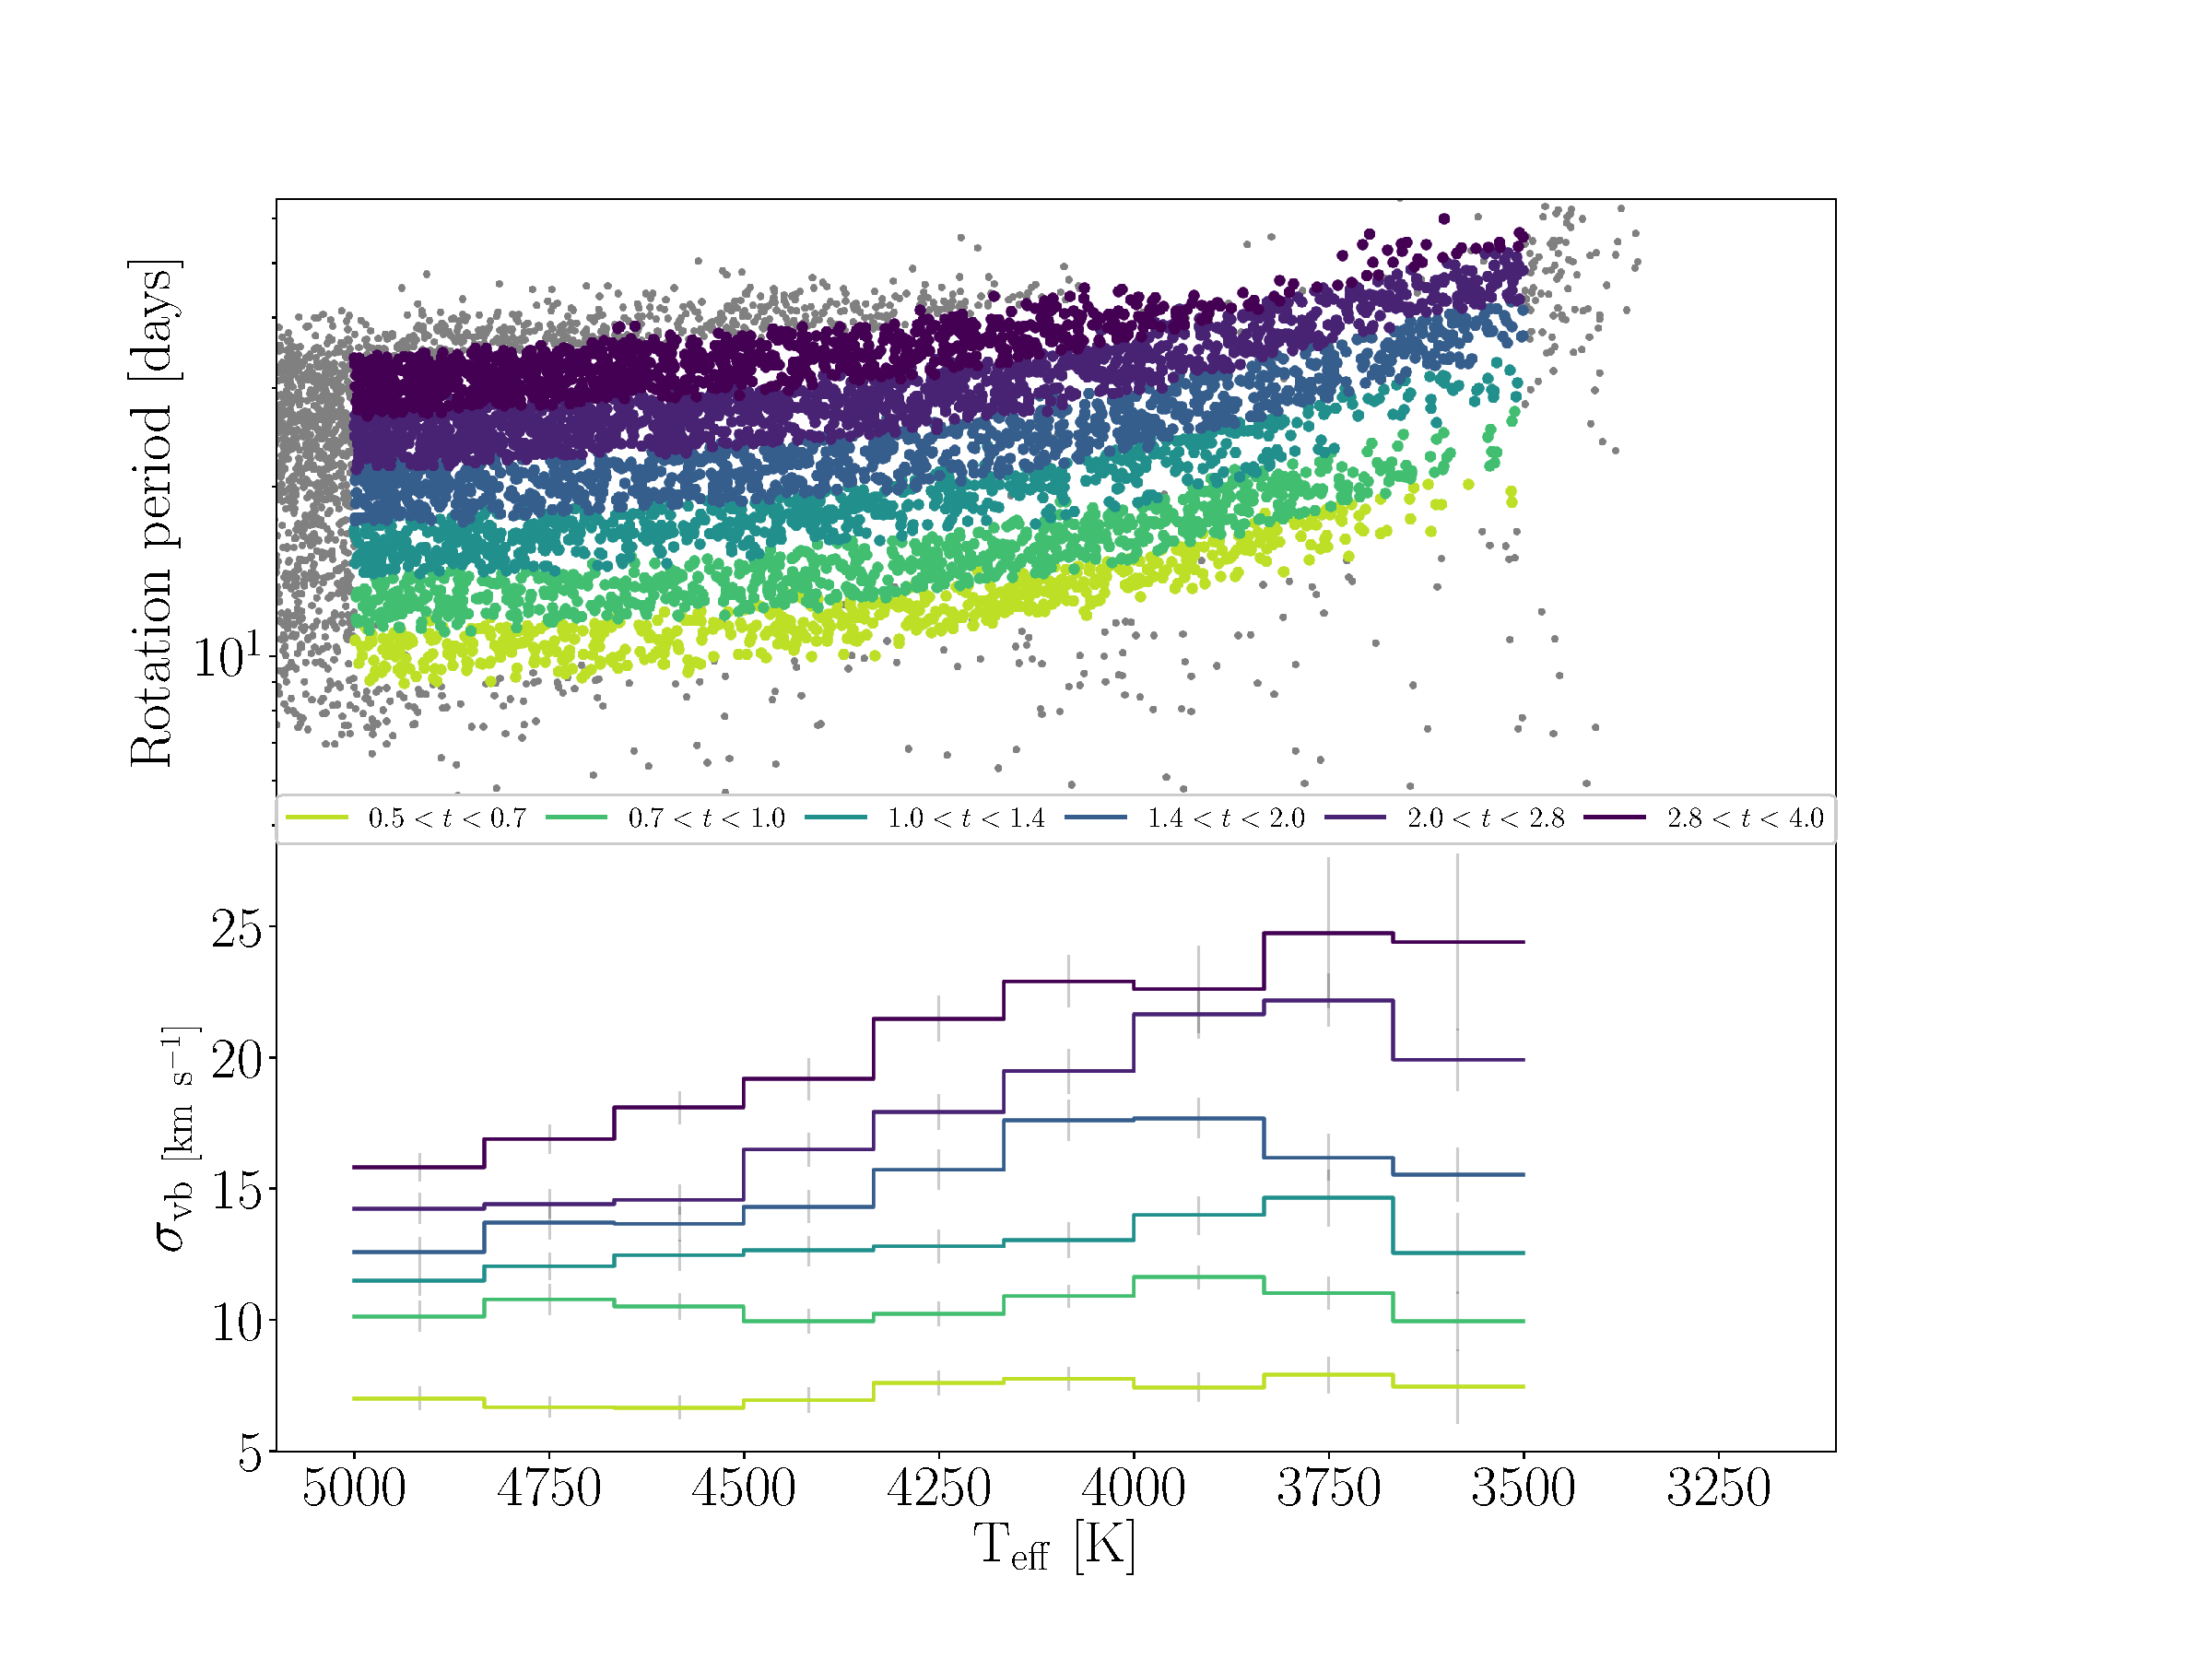
\includegraphics[width=1\textwidth]{age_cut}
\label{fig:age_cut}
\end{figure}
The top panel of figure \ref{fig:age_cut} shows the full \mct\ sample
(excluding visual binaries and subgiants) in grey, with coeval groups shown in
color.
The color of the points corresponds to the age ranges specified in the legend
(in Gyr), which also apply to the lines in the lower panel.
The bottom panel shows the velocity dispersion, \sigmavb\ of each age group,
as a function of effective temperature.
% We only included stars within a temperature range of 5000 - 3500 K in our
% analysis, as hotter stars are more likely to have stopped magnetic braking
% \citep{vansaders2016}, which could bias the results.
% Late M dwarfs were not included in our analysis because such faint stars
% cannot be observed at large heights above the plane (because of the low
% galactic latitude of the \kepler\ field, stars at high-Z are more distant),
% which introduces a mass-dependent velocity bias: cooler populations of stars
% are skewed towards lower velocity dispersions.
% The coolest temperature bins in the lower panel of figure \ref{fig:age_cut}
% have low velocity dispersions, indicating that this effect may already become
% important at temperatures lower than $\sim$ 4000 K.
Overall, figure \ref{fig:age_cut} shows that velocity dispersion increases
with gyrochronal age across all temperatures, implying that both velocity
dispersion and rotation periods increase with age as expected.
The constant velocity dispersion of young stars as a function of temperature
shows that the Praesepe-calibrated gyrochronology relation accurately predicts
the relative ages of {\it young} field stars.
% To our knowledge, no gyrochronology relation has previously been demonstrated to
% correctly predict ages (either relative or absolute) for such cool or such
% young field stars.
% This is not particularly remarkable however, since these young stars are a
% similar age to the Praesepe cluster, which was used to calibrate the
% period-color relation.
% However, if the stars in each selected age group had the {\it same} age across
% the temperature range, their velocity dispersion would be a constant function
% of \teff.
In contrast however, velocity dispersion increases as a function of
temperature for old stars, meaning the \citet{angus2019} gyrochronology
relation either under-predicts the ages of old, late-K dwarfs, or
over-predicts the ages of old early-K and late-G dwarfs\footnote{Since \vb\
velocity dispersion only provides relative and not absolute ages, it is
difficult to tell whether the ages of cool stars are being under-predicted,
the ages of hot stars being are over-predicted, or both.}.
This indicates that the relationship between rotation period and photometric
color or \teff\ flattens out over time, and possibly even inverts.
The lines of constant age (isochrones) sweeping diagonally upwards in the top
panel of figure \ref{fig:age_cut} are too steeply sloped at old ages.

\subsection{The period-\teff\ relations, revealed}
\label{sec:the_reveal}

\begin{figure}
  \caption{
      Top: Rotation period vs effective temperature for stars in the \mct\
    sample, colored by the velocity dispersions of stars calculated over a
    grid in $\log_{10}$(period) and \teff.
    Bottom: the velocity dispersions of groups of stars, shown as a solid
    grid for clarity.
    The hatched area indicates the temperature regime where selection biases
    could play an important role, so these velocity dispersions should be
    interpreted with caution.
    The black solid lines on both panels show a 1.1 Gyr isochrone, calculated
    with the \citet{angus2019} gyrochronology relation, which roughly traces
    the rotation period gap.
    The black dashed lines show a 650 Myr isochrone, indicating the location
    and shape of the Praesepe cluster (to which this gyrochronology model was
    calibrated).
    The black points show the 1.1 Gyr NGC 6811 open cluster.
}
  \centering
    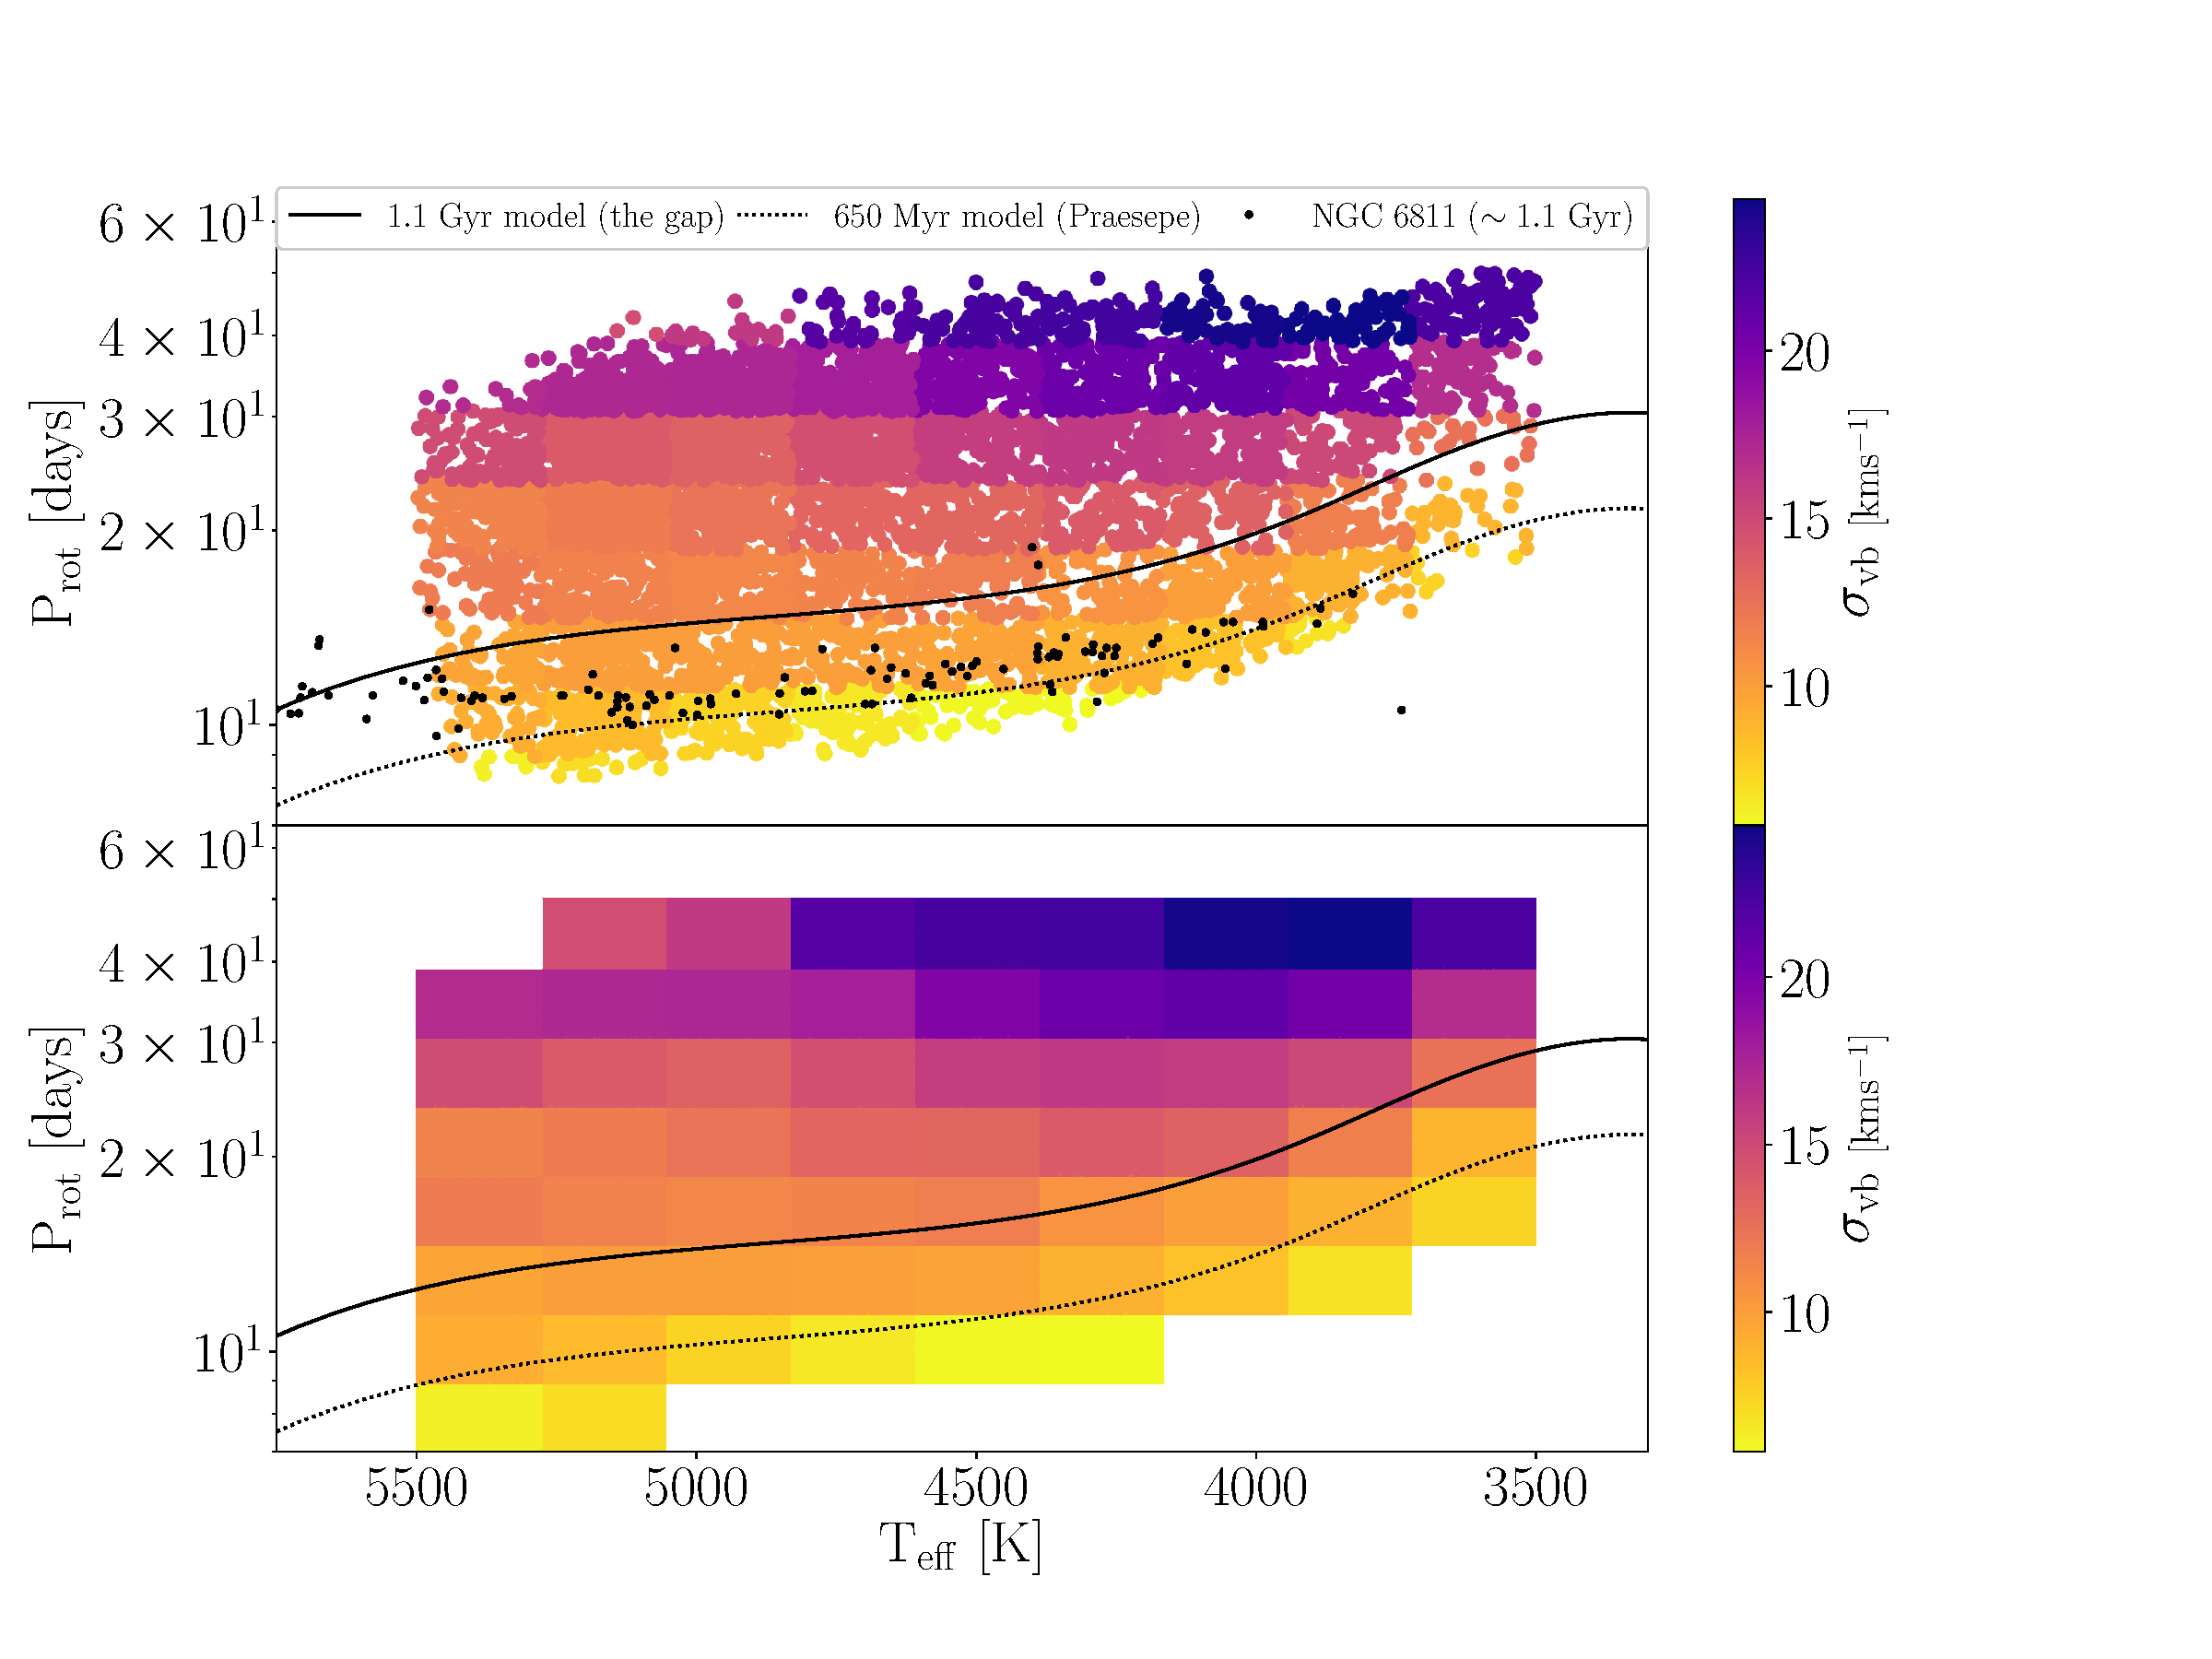
\includegraphics[width=1\textwidth]{vplot}
\label{fig:dispersion_period_teff}
\end{figure}
Figure \ref{fig:dispersion_period_teff} shows rotation period vs. \teff\ for
our sample, coloured by (\vb) velocity dispersion, where \sigmavb\ was
calculated for groups of stars over a grid in $\log_{10}$(period) and
temperature.
If we assume that mass dependent heating does not strongly affect this sample
and \vb\ at low galactic latitudes is an unbiased tracer of \vz, then \vb\
velocity dispersion can be interpreted as an age proxy and stars plotted in a
similar color in figure \ref{fig:dispersion_period_teff} are similar ages.
Interpreted this way, lines of constant age (isochrones) appear to follow the
shape of the Praesepe-based gyrochronology model (black solid and dotted
lines) at young ages.
However, at older ages it appears that the relation between rotation period
and \teff\ flattens out, until eventually rotation period {\it decreases} with
decreasing effective temperature at a given age.

The shape of the period-\teff\ relations at old ages appears to follow the
shape of the upper detection edge.
The so-called `M dwarf dip' \citep{vansaders2018} is reflected in the lines of
constant velocity dispersion (and presumed age) in the top panel of figure
\ref{fig:dispersion_period_teff}.
If the shape of the upper edge of rotation period measurements is created by a
detection limit, it could indicate the rotation periods at which stars of
different temperatures become relatively inactive (and their rotation periods
therefore become undetectable).
% Once inactive, stars would have little photometric variability induced by
% star spots and their rotation periods would be difficult to measure, so may
% not feature in the \mct\ catalog.
If so, figure \ref{fig:dispersion_period_teff} suggests that stars cooler than
$\sim$4500 K become inactive at a similar age, and stay active longer than
stars hotter than $\sim$4500 on average.

% The groups of stars with the largest velocity dispersions are cooler than 4500
% K, presumably because cooler stars remain active for longer, and their
% rotation periods can therefore be measured at older ages.

The velocity dispersions of the coolest stars may be affected by a selection
bias -- these extremely faint stars are more difficult to detect at larger
distances, larger heights above the plane, and therefore larger velocities.
It is possible that some high velocity stars of temperatures cooler than
$\sim$4000 K are missing from this sample, and the velocity dispersions may
therefore appear lower than they truly are.
This could be why the velocity dispersion appears to decrease towards the
right of figure \ref{fig:dispersion_period_teff}.

% \subsection{The period gap}
% \label{sec:period_gap}

% The origin of the rotation period gap, first identified
% by \citet{mcquillan2013} and visible in figures \ref{fig:age_cut} and
% \ref{fig:dispersion_period_teff} still remains a mystery.
% This gap can be seen as an under-density of points between the 0.7-1.0 and
% 1.0-1.5 Gyr age ranges in figure \ref{fig:age_cut} and roughly follows a line
% of constant gyrochronal age of around 1.1 Gyr \citep[according to the
% gyrochronology relation of][]{angus2019}, as shown in figure
% \ref{fig:dispersion_period_teff}.
% Several explanations for the gap's origin have been proposed, including a
% discontinuous star formation history \citep{mcquillan2013, davenport2017,
% davenport2018}, a rapid change in magnetic field structure
% \citep{reinhold2019}, and erroneous rotation period measurements that are
% incorrect by a factor of two \citep{koen2018}.
% The latter explanation can be ruled out because stars below the gap have
% smaller velocity dispersions than the stars above the gap, indicating that
% they are kinematically younger \citep{mcquillan2013, davenport2018}, as
% evident in figures \ref{fig:age_cut} and \ref{fig:dispersion_period_teff}.
% For stars below the gap, in the 0.7-1.0 Gyr age range shown in figure
% \ref{fig:age_cut}, velocity dispersion is relatively constant as a function of
% temperature, however above the gap, in the 1.0-1.5 Gyr age range and older,
% velocity dispersion increases with \teff.
% The coolest stars in the 1.0-1.5 Gyr age range have the same velocity
% dispersion as the hottest stars in the age range above which indicates that
% the period-\teff\ relations are {\it flat} at these rotation periods.
% This is also visible in figure \ref{fig:dispersion_period_teff}.
% Below the gap, velocity dispersion within a given period range appears to {\it
% decrease} with decreasing temperature.
% The opposite appears to be true above the gap.
% It could be that the gap is positioned at a significant Rossby number/age at
% which stellar magnetic dynamos go through a transition.
% Perhaps before the age of 1.1 Gyr, or at Rossby numbers less than ???,
% magnetic braking is more efficient for stars with deeper convection zones.
% Once stars reach this critical age or Rossby number their magnetic fields
% undergo some radical transition, which produces the gap in the rotation
% period-\teff\ plane.
% After this transition, magnetic braking efficiency no longer increases with
% decreasing mass.
% Of course, it may be a coincidence that the gyrochronology relations seem to
% only flatten off above the period gap and we lack a sufficient quantity of
% data to do more than speculate here.
% New rotation periods from the \ktwo\ and \tess\ missions may be able to
% validate or rule out this hypothesis in the future.

% In the $\sim$ 1.1 Gyr NGC 6811 cluster, the rotation periods of mid-K dwarfs
% are faster than expected; their rotational evolution appears to have stalled,
% and they have similar rotation periods to the 650 Myr Praesepe cluster
% \citep{curtis2019}.
% The rotation periods of the K dwarfs in this cluster are plotted in figure
% \ref{fig:dispersion_period_teff}.
% Although NGC 6811's G dwarfs fall on the 1.1 Gyr gyrochronology model, the K
% dwarfs lie only a little above the 0.65 Gyr gyrochronology model.
% NGC 6811 straddles the rotation period gap: its G dwarfs lie above it and its
% K dwarfs lie below it.
% This cluster may be the `missing link' that connects two epoch of stellar
% spin-down.
% % , however without more observations of middle-aged open clusters it
% % : an early stage where the period-\teff\ relation for cool dwarfs has
% % a negative slope and a late stage where it has a positive slope.
% % In this case the period gap may delineate the transition between these two
% % regimes and is the point at which stellar magnetic dynamos likely undergo a
% % dramatic structural shift at an age of $\sim$ 1.1 Gyr.
